% Intended LaTeX compiler: pdflatex
\documentclass[10pt,a4paper,UTF8]{article}
\usepackage{zclorg}
\usepackage{tikztheorem}
\author{zcl.space}
\date{}
\title{Axioms for the Real Numbers}
\hypersetup{
 pdfauthor={zcl.space},
 pdftitle={Axioms for the Real Numbers},
 pdfkeywords={PMA},
 pdfsubject={},
 pdfcreator={Emacs 25.0.50.1 (Org mode 9.1.2)},
 pdflang={English}}
\begin{document}

\maketitle
\tableofcontents
\titlepic{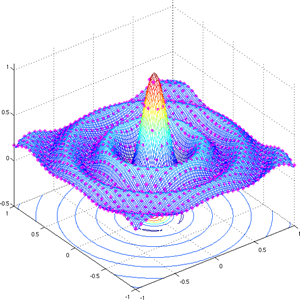
\includegraphics[scale=0.25]{../../img/sinc.PNG}}
We state here the axioms for the real number system \(\mathbb{R}\).
We shall accept these axioms without proof but
it can proved (from more general axioms)
that there is an essentially unique structure satisfying them.


\textbf{Algebraic Axioms} .
The set \(\mathbb{R}\) of \textbf{real numbers}  is equipped with two operations
$$
\mathbb{R}\times\mathbb{R}\to\mathbb{R}:(a,b)\mapsto a+b,\qquad\mathbb{R}\times\mathbb{R}\to\mathbb{R}:(a,b)\mapsto a\cdot b
$$
such that the usual laws of grade school arithmetic hold:

\begin{enumerate}
\item \textbf{Commutative Laws} \(a+b=b+a\) and \(a\cdot b=b\cdot a\).
\item \textbf{Associative Laws}  \((a+b)+c=a+(b+c)\) and \((a\cdot b)\cdot c= a\cdot (b\cdot c)\).
\item \textbf{Distributive Law} \((a+b)\cdot c= (a\cdot c)+(b\cdot c)\).
\item \textbf{Zero,One} There are (necessarily unique) distinct elements \(0,1\in\mathbb{R}\) such that \(a+0=a\) and \(a\cdot 1=a\) for all \(a\in\mathbb{R}\).
\item \textbf{Inverses} For every \(a\in\mathbb{R}\) there is a (necessarily unique) element \(-a\) such that \(a+(-a)=0\). For every \(a\in\mathbb{R}\setminus\{0\}\) there is a (necessarily unique) element \(a^{-1}\) such that \(a\cdot a^{-1}=1\).
\end{enumerate}

The standard notations from high school algebra are used:
 in particular, \(ab:=a\cdot b\), \(a-b:=a+(-b)\), and \(a/b=a\cdot b^{-1}\).


\textbf{Order Axioms} .   The set \(\mathbb{R}\) has an order relation
denoted \$ a < b\$ satisfying the following laws for all \(a,b,c\in\mathbb{R}\):

\textbf{Trichotomy}   Exactly one of the alternatives    \$ a < b\$, \(a=b\), \(b < a\), holds.
\textbf{Transitivity}    \(a < b,\;b < c\implies a < c\).
\textbf{Addition}    \(a < b\implies a+c < b+c\).
\textbf{Multiplication}     \(0 < a,b\implies 0 < ab\).

The other order notations are defined as usual, i.e.
\(a < b\iff b>a\) and \(a\le b\iff b\ge a\iff\) either \(a < b\) or \(a=b\).


All the rules of algebra used in College Algebra
 follow from the Algebraic Axioms and Order Axioms.
For example, \((a+b)^2=a^2+2ab+b^2\), \(a^2\ge 0\), etc.


A set \(S\)  of real numbers is said to be \textbf{bounded above} iff there is
a  number \(b\in\mathbb{R}\) such that \$x\(\le\) b \$ for all \(x\in S\);
the number \(b\) is  then called an \textbf{upper bound}  for \(S\).
A number \(b\in\mathbb{R}\) is called a \textbf{least upper bound}  for \(S\) iff
it is an upper bound for \(S\) and
\(b\le b'\) for every other upper bound \(b'\) for \(S\).

 Similarly  the set \(S\) is said to be \textbf{bounded below}  iff there is
an number \(a\in\mathbb{R}\) such that \(a\le x\) for all \(x\in S\);
the element \(b\) is  then called a  \textbf{lower bound}  for \(S\).

An element \(a\in\mathbb{R}\) is called a \textbf{greatest lower bound}
iff it is an lower bound for \(S\) and  \(a'\le a\) for every other lower bound
\(a'\) for \(S\).  The words \textbf{infimum}  and \textbf{greatest lower bound} are synonymous
as are the   words \textbf{supremum}  and \textbf{least upper bound}.
The least upperbound of the set \(S\) will be denoted \(\sup(S)\)
and
the greatest lower bound of the set \(S\) will be denoted \(\inf(S)\).
We write \(\sup(S)=\infty\) when \(S\) is not bounded above and \(\inf(S)=-\infty\)
when \(S\) is not bounded below.


\textbf{Completeness Axiom} .
Every set \(S\) of real numbers which is bounded above has a least upper bound, i.e.

if \(x\le b\) for all \(x\in S\), then \(x\le \sup(S)\le b\) for all \(x\in S\).

Because multiplication by \(-1\) reverses the order it is the same to say that every set which is bounded below has a greatest lower bound. Thus

if \(a\le x\) for all \(x\in S\), then
\(a\le \inf(S)\le x\) for all \(x\in S\).

For Morgan the completeness axiom is a theorem (see page\textasciitilde{}44 of his book)
but most authors of undergraduate texts don't prove it.
Of course it can't be proved until we give a precise construction (definition)
of the real numbers.

Morgan takes the view that a real number is a number with
a decimal expansion, but avoids certain subtle issues connected
with this view.

Actually making his definition precise would involve defining how to do
the arithmetic operations with decimal expansions and would be
a bit tedious.  To see why, imagine that \(a+b=c\) and that
$$
  a=\sum_{n=1}^\infty a_n10^{-n},\qquad
  b=\sum_{n=1}^\infty b_n10^{-n},\qquad
  c=\sum_{n=1}^\infty c_n10^{-n},
$$
where the coefficients, \(a_n,b_n,c_n\) are integers between \(0\) and \(9\)
and try to express \(c_n\) in terms the \(a_n\)'s and the \(b_n\)'s.
In an appendix to his book, Buck sketches a construction the real numbers
by something called \textbf{Dedekind cuts}   but leaves out many details.
Rudin explains cuts in an appendix to his chapter\textasciitilde{}1.
(The book \{\em Foundations of Analysis\} by Edmund Landau gives all the details.)
The completeness axiom is an easy consequence of this construction.
One can also define the real numbers using `equivalence classes of Cauchy sequences'
 and again the completeness axiom is a consequence;

if we get to the topic of completion of metric spaces, I'll explain it then.

The crucial point is the uniqueness `up to isomorphism'.

It means that if we start from  the axioms, it doesn't matter what
definition of the real numbers we use.
\end{document}
